\documentclass[convert={outfile=\jobname.svg}]{standalone}
\usepackage[dvipsnames]{xcolor}
\usepackage{tikz}
\usetikzlibrary{calc}
\tikzset{dot/.style={draw,shape=circle,fill=black,scale=0.4}}
\usepackage[outline]{contour}
\contourlength{0.05em}
\newcommand{\outline}[1]{\contour*{white}{#1}}

% Correctly centred vdots.
\newcommand{\tri}{\draw (90:1) -- (210:1) -- (330:1) -- cycle;}

\begin{document}
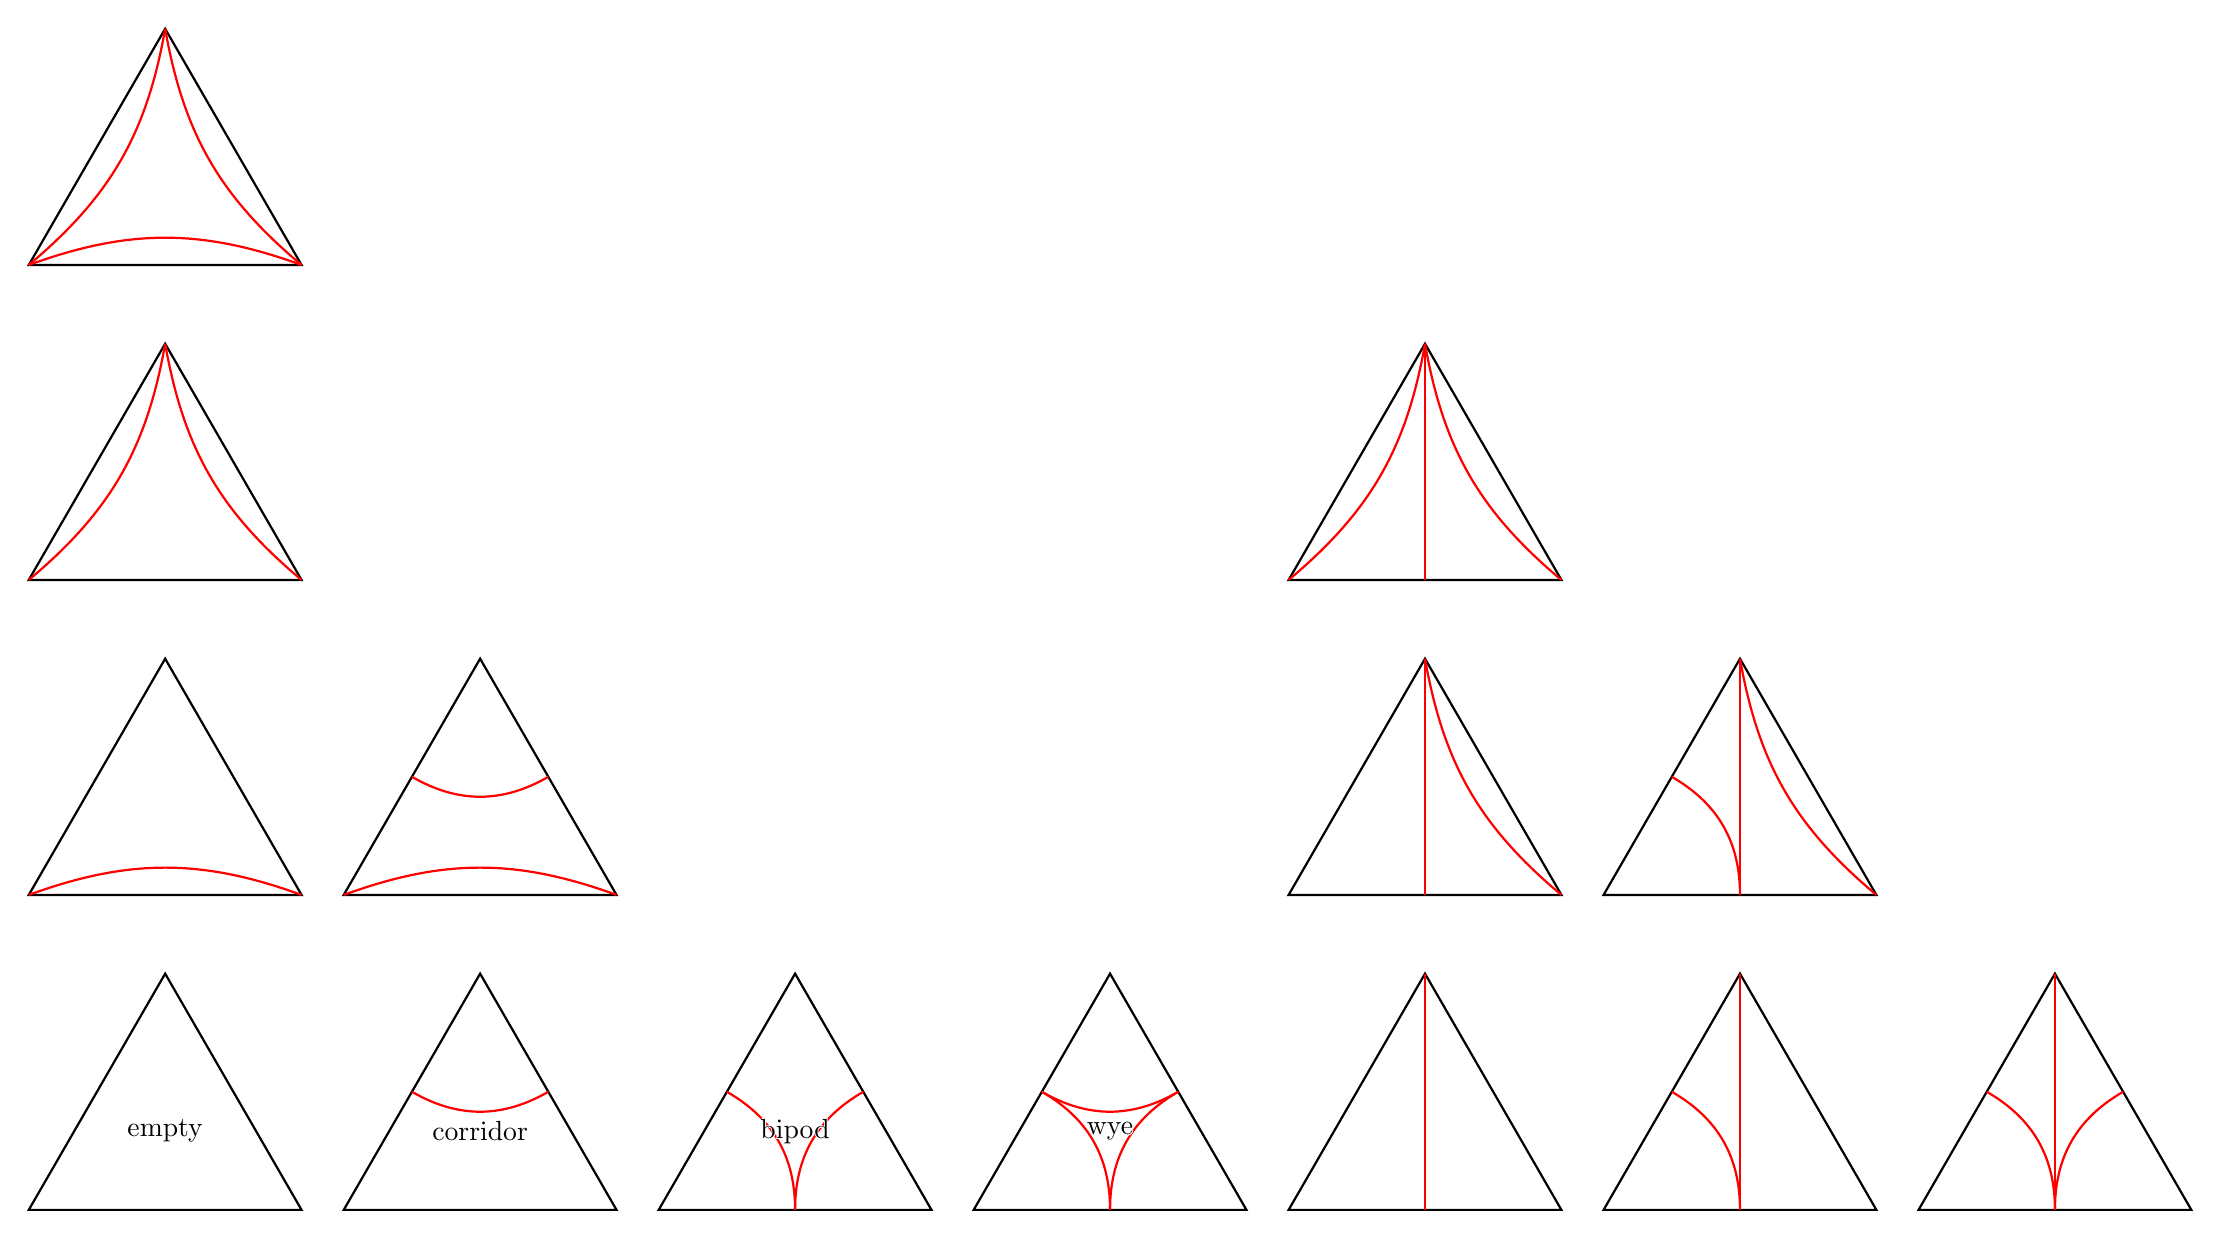
\begin{tikzpicture}[scale=2, thick]
    \begin{scope}[shift={(0, 0)}]
    \tri{}
    \node at (0,0) {empty};
    \end{scope}
    
    \begin{scope}[shift={(2, 0)}]
    \tri{}
    \draw [red] ($(90:1)!0.5!(210:1)$) to [out=330,in=210] ($(90:1)!0.5!(330:1)$);
    \node at (0,0) {corridor};
    \end{scope}
    
    \begin{scope}[shift={(4, 0)}]
    \tri{}
    \draw [red] ($(90:1)!0.5!(210:1)$) to [out=330,in=90] ($(210:1)!0.5!(330:1)$);
    \draw [red] ($(90:1)!0.5!(330:1)$) to [out=210,in=90] ($(210:1)!0.5!(330:1)$);
    \node at (0,0) {\outline{bipod}};
    \end{scope}
    
    \begin{scope}[shift={(6, 0)}]
    \tri{}
    \draw [red] ($(90:1)!0.5!(210:1)$) to [out=330,in=90] ($(210:1)!0.5!(330:1)$);
    \draw [red] ($(90:1)!0.5!(330:1)$) to [out=210,in=90] ($(210:1)!0.5!(330:1)$);
    \draw [red] ($(90:1)!0.5!(210:1)$) to [out=330,in=210] ($(90:1)!0.5!(330:1)$);
    \node at (0,0) {\outline{wye}};
    \end{scope}
    
    \begin{scope}[shift={(8, 0)}]
    \tri{}
    \draw [red] (90:1) to [out=270,in=90] ($(210:1)!0.5!(330:1)$);
    \end{scope}
    
    \begin{scope}[shift={(10, 0)}]
    \tri{}
    \draw [red] (90:1) to [out=270,in=90] ($(210:1)!0.5!(330:1)$);
    \draw [red] ($(90:1)!0.5!(210:1)$) to [out=330,in=90] ($(210:1)!0.5!(330:1)$);
    \end{scope}
    
    \begin{scope}[shift={(12, 0)}]
    \tri{}
    \draw [red] (90:1) to [out=270,in=90] ($(210:1)!0.5!(330:1)$);
    \draw [red] ($(90:1)!0.5!(210:1)$) to [out=330,in=90] ($(210:1)!0.5!(330:1)$);
    \draw [red] ($(90:1)!0.5!(330:1)$) to [out=210,in=90] ($(210:1)!0.5!(330:1)$);
    \end{scope}
    
    \begin{scope}[shift={(0, 2)}]
    \tri{}
    \draw [red] (210:1) to [out=20,in=160] (330:1);
    \end{scope}
    
    \begin{scope}[shift={(0, 4)}]
    \tri{}
    \draw [red] (90:1) to [out=260,in=40] (210:1);
    \draw [red] (90:1) to [out=280,in=140] (330:1);
    \end{scope}
    
    \begin{scope}[shift={(0, 6)}]
    \tri{}
    \draw [red] (210:1) to [out=20,in=160] (330:1);
    \draw [red] (90:1) to [out=260,in=40] (210:1);
    \draw [red] (90:1) to [out=280,in=140] (330:1);
    \end{scope}
    
    \begin{scope}[shift={(2, 2)}]
    \tri{}
    \draw [red] ($(90:1)!0.5!(210:1)$) to [out=330,in=210] ($(90:1)!0.5!(330:1)$);
    \draw [red] (210:1) to [out=20,in=160] (330:1);
    \end{scope}
    
    \begin{scope}[shift={(8, 2)}]
    \tri{}
    \draw [red] (90:1) to [out=270,in=90] ($(210:1)!0.5!(330:1)$);
    \draw [red] (90:1) to [out=280,in=140] (330:1);
    \end{scope}
    
    \begin{scope}[shift={(8, 4)}]
    \tri{}
    \draw [red] (90:1) to [out=270,in=90] ($(210:1)!0.5!(330:1)$);
    \draw [red] (90:1) to [out=280,in=140] (330:1);
    \draw [red] (90:1) to [out=260,in=40] (210:1);
    \end{scope}
    
    \begin{scope}[shift={(10, 2)}]
    \tri{}
    \draw [red] (90:1) to [out=270,in=90] ($(210:1)!0.5!(330:1)$);
    \draw [red] ($(90:1)!0.5!(210:1)$) to [out=330,in=90] ($(210:1)!0.5!(330:1)$);
    \draw [red] (90:1) to [out=280,in=140] (330:1);
    \end{scope}
\end{tikzpicture}
\end{document}
